\chapter{Methodology}

The development of Aether Co-Pilot followed a structured yet flexible Agile methodology to account for the iterative nature of AI feature development. Agile methodology provides continuous iteration of development and testing throughout the software development lifecycle of the project. It emphasizes a pragmatic approach, focusing on delivering working software quickly while remaining open to requirement changes as feedback is collected. Our approach utilized two-week sprints, starting with fundamental research into Large Language Models, followed by UI prototyping in Figma, and culminating in concurrent module programming.

\section{System Architecture}

The system architecture is designed as a hybrid cloud-native environment. It separates the client interface, identity management, database persistence, and AI inference into distinct layers, ensuring that bottlenecks in one system do not halt the entire application.

\begin{figure}[!ht]
\centering
% \includegraphics[width=0.9\textwidth]{images/architecture.png}
% Placeholder for user image. If image does not exist, pdflatex error handles or skips.
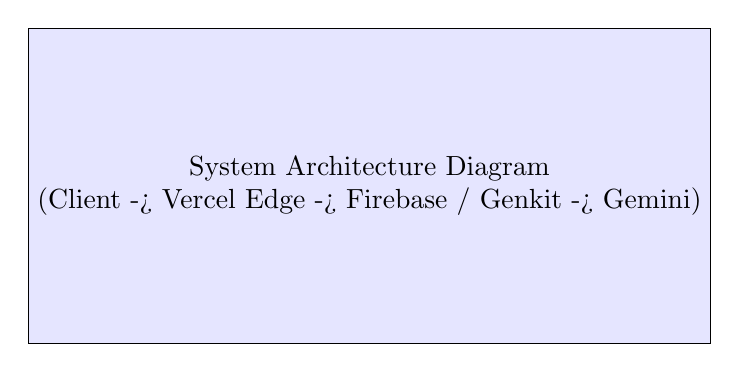
\begin{tikzpicture}
  \node[draw, rectangle, minimum width=8cm, minimum height=4cm, align=center, fill=blue!10] {System Architecture Diagram \\ (Client -> Vercel Edge -> Firebase / Genkit -> Gemini)};
\end{tikzpicture}
\caption{Overall System Architecture for Aether Co-Pilot}
\label{fig:sys_arch}
\end{figure}

The architecture utilizes Next.js deployed on Vercel's Edge network for initial client requests. Static assets are served globally, while dynamic AI queries are routed to Firebase Cloud functions running Google Genkit. Genkit acts as the orchestrator, validating prompts, fetching context from Firestore, and ultimately performing inference using the Gemini 2.0 Flash model.

\section{Module}

The system is decomposed into a series of independently testable functional modules.

\subsection{1. user registration module}
The user registration module allows new individuals to create an account on the Aether platform. It integrates securely with Clerk to hash credentials and issue initial authentication tokens. Upon successful registration, a webhook triggers the creation of a corresponding user document within our private Firestore instance to securely house future data.

\subsection{2. Login and authentication Module}
The login module handles recurring access to the platform. It intercepts all incoming requests and verifies the status of the JSON Web Token (JWT). If the token is expired or missing, the user is redirected to the login interface. It also seamlessly syncs the Clerk identity token to a custom Firebase authentication token to establish dual-layer security.

\subsection{Modules of Aether Co-pilot}
Beyond basic identity management, the Aether ecosystem relies on highly specialized modules:
\begin{itemize}
    \item \textbf{Cognitive Memory Core (Chat Module)}: Manages the context windows for users, storing previous interactions and retrieving them via semantic search when answering new queries.
    \item \textbf{Quantum CodeForge (Coding Module)}: Specialized prompt engineering module focused purely on taking voice or text inputs and translating them precisely into executable Javascript, Python, or TypeScript code blocks.
    \item \textbf{Knowledge Navigator (Study Module)}: A robust file ingestion module that parses PDF and text data, creates embeddings, and performs localized Retrieval-Augmented Generation (RAG) for student inquiries.
    \item \textbf{Task Automation Engine (Automation Module)}: Analyzes plain English requests and synthesizes corresponding terminal commands (e.g., shell scripts) to automate redundant operating system or web tasks.
\end{itemize}

\newpage
